\documentclass[12pt,letterpaper,noanswers]{exam}
\usepackage[usenames,dvipsnames,svgnames,table]{xcolor}
\usepackage[margin=0.9in]{geometry}
\renewcommand{\familydefault}{\sfdefault}
\usepackage{multicol}
\pagestyle{head}
\definecolor{c03}{HTML}{FFDDDD}
\header{AM 108 Class 04}{Updated on \today.}{Sept 9: Bifurcations}
\runningheadrule
\headrule
\usepackage{graphicx} % more modern
\usepackage{amsmath} 
\usepackage{amssymb} 
\usepackage{hyperref}
\usepackage{tcolorbox}

\begin{document}
 \pdfpageheight 11in 
  \pdfpagewidth 8.5in

\vspace{0.2cm}

\hrule
\vspace{0.2cm}

\begin{itemize}
    \item There is be a pre-class assignment for Monday (Check Yourself C05).
    \item There is a one question skill check on Monday.  The sample question for it is below.
    \item Before attending OH, post to \#officehours on Slack (or the Office Hours thread on Piazza) to let your classmates and the course staff know what questions / problems you're bringing to OH.
    \item Problem Set 02 will be posted by middate on Saturday.
\end{itemize}

\hrule
\vspace{0.2cm}

\noindent\textbf{Teams}

We will switch to new teams on Monday.  

\begin{multicols}{2}
1. 
\end{multicols}

\noindent \textbf{Teams 2 and 3}: Post screenshots of your work to the course Google Drive today.  Include words, labels, and other short notes that might make those solutions useful to you or your classmates.  Find the link in Canvas (or here: \url{https://drive.google.com/drive/u/0/folders/1GcpwvKHD4tMecpFQ4lNxN_r5Ylj7YHbd})

\vspace{0.2cm}
\hrule
\vspace{0.2cm}

\noindent\textbf{Desmos}.

Consider $\dot x = r x - \tanh x$.  It is important to know how to make the plot by hand.

Using Desmos can also be helpful when you are plotting with parameters.

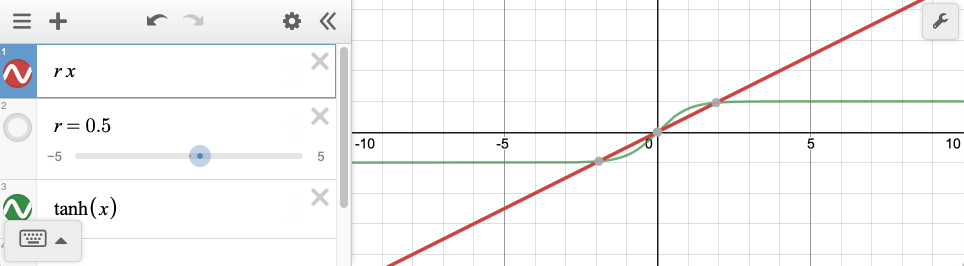
\includegraphics[width = 0.5\linewidth]{img/C04desmosp3.png}

\vspace{0.2cm}
\hrule
\vspace{0.2cm}

\noindent Skill Check interlude.

\vspace{0.2cm}
\hrule
\vspace{0.2cm}

\noindent \textbf{Introduction to maps:}

definitions from Alligood, Sauer, Yorke. 2012. \underline{Chaos: An introduction to dynamical systems}
\begin{tcolorbox}

We'll use the term \textbf{map} for a function whose domain (input space) and range (output space) are the same. 

Let $x$ be a point and $f$ be a map.  The \textbf{orbit} of $x$ under $f$ is the set of points $\{x, f(x), f^2(x),...\}$.  

The starting point $x$ for the orbit is called the \textbf{initial value} of the orbit.  

A point $p$ is a \textbf{fixed point} of the map $f$ if $f(p) = p$.
\end{tcolorbox}
\vfill

% \vspace{0.2cm}

% \hrule
% \vspace{0.2cm}
\eject
\noindent\textbf{Finding orbits graphically}:

\begin{tcolorbox}
We use a \textbf{cobweb plot} to find orbits graphically.  To make the plot: \begin{enumerate}
\itemsep0em
    \item Start at $(x,x)$ or $(x,0)$ and draw a vertical line to $(x,f(x))$.  Our partial orbit is now $\{x, f(x)\}$.
    \item Draw a horizontal line from $(x,f(x))$ to $(f(x),f(x))$.
    \item Draw a vertical line from $(f(x),f(x))$ to $(f(x), f^2(x))$.  Our partial orbit is now $\{x, f(x), f(f(x))\}$.
    \item Alternate drawing horizontal and vertical lines.  Horizontal lines go to the point $(f^k(x),f^k(x))$ and vertical lines go to the point $(f^k(x), f^{k+1}(x))$ (so vertical lines show us the next element of the orbit).
\end{enumerate} 
\end{tcolorbox}

\noindent\textbf{Example}.  $x_{n+1} = f(x_n)$ with $f(x) = 2x(1-x)$.  

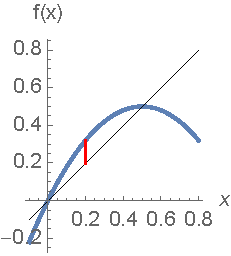
\includegraphics{img/C04mapsp1.pdf}
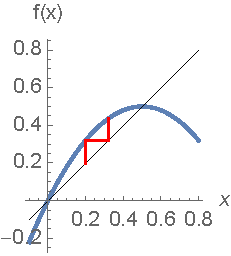
\includegraphics{img/C04mapsp1b.pdf}
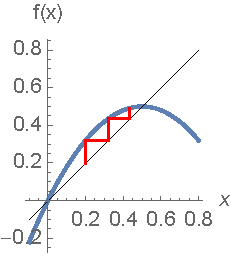
\includegraphics{img/C04mapsp1c.pdf}
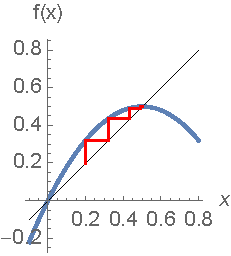
\includegraphics{img/C04mapsp1d.pdf}

\vspace{2in}

\noindent\textbf{Practice}.


Write your names on your Jamboard slide before you begin.


Let $x_{n+1} = f(x_n)$ with $f(x) = \cos x$.
\begin{itemize}
\itemsep0em
    \item Plot $\cos x$ and $x$ on the same plot.
    \item Use your plot to identify any fixed points of the map.
    \item Make cobwebs for at least two qualitatively different cases.
\end{itemize}

\eject

\vspace{0.2cm}
\hrule
\vspace{0.2cm}

\noindent\textbf{Stability of fixed points}:

\begin{tcolorbox}
Let $f$ be a map on $\mathbb{R}$ and let $p$ be a real number such that $f(p) = p$.  We call $p$ an \textbf{attracting fixed point}, a \textbf{sink}, or a \textbf{stable fixed point}, if all points sufficiently close to $p$ are attracted to $p$. \\

We call $p$ a \textbf{repelling fixed point}, a \textbf{source}, or an \textbf{unstable fixed point}, if all points sufficiently close to $p$ are repelled from $p$. 
\end{tcolorbox}

\noindent\textbf{Stability condition?}

In maps, we can formulate an analytic stability condition, just as we did for flows.  For the following four examples, we have $f'(x^*) = 0.5, -0.5, 1.5, -1.5$.  Use cobwebbing to identify the stability of the fixed point in each example.

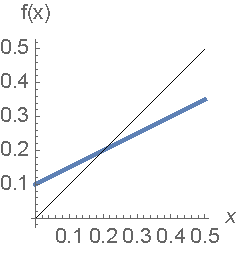
\includegraphics{img/C04mapsp3a.pdf}
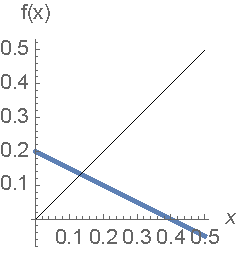
\includegraphics{img/C04mapsp3b.pdf}
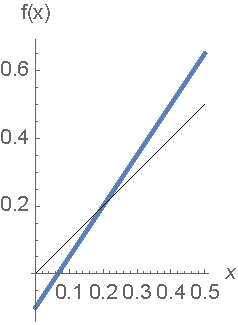
\includegraphics{img/C04mapsp3c.pdf}
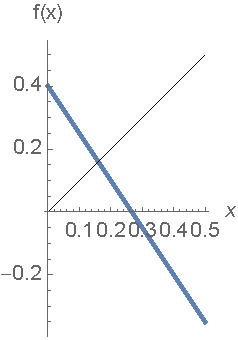
\includegraphics{img/C04mapsp3d.pdf}

\vspace{2in}

\vspace{0.2cm}
\hrule
\vspace{0.2cm}

\noindent\textbf{Bifurcations}:
\begin{tcolorbox}
Just as in our work with flows, in maps fixed points typically change stability at \textbf{bifurcation points}.

One type of bifurcation occurs when $f'(x^*) = 1$.  A different type occurs when $f'(x^*) = -1$.
\end{tcolorbox}


\vspace{0.2cm}
\hrule
\vspace{0.2cm}
\eject



\vspace{0.2cm}
\hrule
\vspace{0.2cm}

\noindent\textbf{Skill check C05 practice} (the skill check for C05 on Monday will have one question similar, but not identical, to the question below).


\begin{questions}
\item Let $x_{n+1} = f(x_n)$ where $f(x) = 2.3x(1-x)$.  Add a cobweb to the graph, using the red dot as your starting value of $x$.

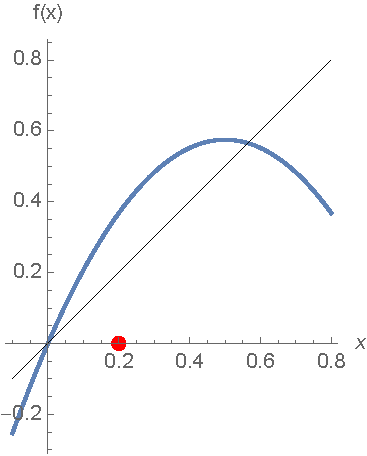
\includegraphics{img/C04-C05cobweb.pdf}

\end{questions}

\vspace{0.2cm}
\hrule
\vspace{0.2cm}
\noindent\textbf{Skill check C05 practice solution} 

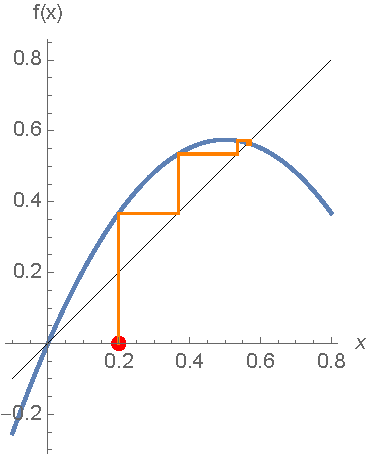
\includegraphics{img/C04-C05cobwebsoln.pdf}

\vspace{0.2cm}

\hrule
\vspace{0.2cm}
\eject

\begin{questions}
\question (9.4.2) The tent map is a simple map
Let \[
x_{n+1} = \left\{
        \begin{array}{ll}
            2x_n, & \quad 0\leq x_n \leq \frac{1}{2} \\
            2-2x_n, & \quad \frac{1}{2}\leq x_n \leq 1.
        \end{array}
    \right.
    \]
    \begin{parts}
    \item Draw $f(x)$ where $x_{n+1} = f(x_n)$.  How many times does it intersect the curve $y=x$?  Why is this map the ``tent map''?
    \item Find the fixed points of this map.
    \item Classify the stability of the fixed points.
    \item Sketch the graph of $f(f(x))$.  How many times does it intersect the curve $y = x$?
    % \item Show the map has a period-$2$ orbit.  This means that there is an $x$ such that $f(f(x)) = x$.
    % \item Classify the stability of any period-$2$ orbits.
    % \item Look for a period-$3$ or period-$4$ point.  If you find one, are such orbits stable or unstable?
    % \item If you want, you can think about whether there is a period-$k$ orbit...
    \end{parts}
\end{questions}













\end{document}